\documentclass[dvipsnames, svgnames, x11names, a4paper, 11pt]{article}

% URLs and hyperlinks ---------------------------------------
\usepackage{hyperref}
\hypersetup{
    colorlinks=true,
    linkcolor=NavyBlue,
    filecolor=magenta,      
    urlcolor=blue,
}
\usepackage{xurl}
%---------------------------------------------------

\usepackage{graphicx}
\usepackage{listings}
\usepackage{color}
\usepackage{xcolor}

\definecolor{dkgreen}{rgb}{0,0.6,0}
\definecolor{gray}{rgb}{0.5,0.5,0.5}
\definecolor{mauve}{rgb}{0.58,0,0.82}

\lstset{frame=tb,
    language=vhdl,
    aboveskip=3mm,
    belowskip=3mm,
    showstringspaces=false,
    columns=flexible,
    basicstyle=\ttfamily,
    numbers=left,
    numberstyle=\small\color{gray},
    keywordstyle=\bfseries\color{Green4},
    commentstyle=\color{gray},
    stringstyle=\color{mauve},
    breaklines=true,
    breakatwhitespace=true,
    tabsize=4,
    identifierstyle=\color{black}
}

\title{Simple ALU}
\author{Mahdi Haghverdi}

\begin{document}
    \maketitle
    \tableofcontents
\section{ALU}
This ALU works but I didn't find a good solution to handle \textbf{overflow} and \textbf{carry/borrow} detection. The rest of the needed functionality works.
\begin{lstlisting}
library ieee;
use ieee.std_logic_1164.all;
use ieee.numeric_std.all;


entity ALU is
    port (
        a, b: in std_logic_vector(31 downto 0);
        m   : in std_logic_vector (3 downto 0);
        s   : out std_logic_vector(31 downto 0);
        z, c, ovf: out std_logic
);
end ALU;

architecture arch of ALU is
begin
process(m, a, b) is
begin
    z <= '0';
    ovf <= '0';
    c <= '0';

    case m is
        when "0000" =>  -- add
            s <= std_logic_vector(signed(a) + signed(b));
        when "0001" =>  -- addu
            s <= std_logic_vector(unsigned(a) + unsigned(b));
        when "0010" =>  -- sub
            if signed(a) = signed(b) then
                z <= '1';
            else
                z <= '0';
            end if;
                s <= std_logic_vector(signed(a) - signed(b));
        when "0011" =>  -- subu
            s <= std_logic_vector(unsigned(a) - unsigned(b));
        when "0100" =>  -- slt
            if signed(a) < signed(b) then
                s <= (0 => '1', others => '0');
            else
                s <= (others => '0');
            end if;
        when "0101" =>  -- sltu
            if unsigned(a) < unsigned(b) then
                s <= (0 => '1', others => '0');
            else
                s <= (others => '0');
            end if;
        when "0110" =>  -- and
            s <= a and b;
        when "0111" =>  -- or
            s <= a or b;
        when "1000" =>  -- nor
            s <= a nor b;
        when "1001" =>  -- xor
            s <= a xor b;
        when others =>
            s <= (others => 'U');
    end case;
end process;
end arch;
\end{lstlisting}

\section{Testbench}
\begin{lstlisting}
library ieee;
use ieee.std_logic_1164.all;
use ieee.numeric_std.all;

entity alu_tb is
end alu_tb;

architecture tb of alu_tb is
    signal a, b: std_logic_vector(31 downto 0);
    signal m   : std_logic_vector (3 downto 0);
    signal s   : std_logic_vector(31 downto 0);
    signal z, c, ovf: std_logic;

begin
    UUT : entity work.alu port map (
        a => a,
        b => b,
        m => m,
        s => s,
        z => z,
        c => c,
        ovf => ovf
    );

m <= "0000",
      "0001" after 20 ns,
      "0010" after 40 ns,
      "0011" after 60 ns,
      "0100" after 80 ns,
      "0101" after 100 ns,
      "0110" after 120 ns,
      "0111" after 140 ns,
      "1000" after 160 ns,
      "1001" after 180 ns,
      "1001" after 200 ns;

a <= "00000000000000000000000000000000",
      "00000000000000000000000000000011" after 20 ns,  -- add
      "00000000000000000000000000000011" after 40 ns,  -- addu
      "00000000000000000000000000000011" after 60 ns,  -- sub
      "00000000000000000000000000000011" after 80 ns,  -- subu
      "00000000000000000000000000000011" after 100 ns, -- slt
      "00000000000000000000000000000011" after 120 ns, -- sltu
      "00000000000000000000000000000011" after 140 ns, -- and
      "00000000000000000000000000000011" after 160 ns, -- or
      "00000000000000000000000000000011" after 180 ns, -- nor
      "00000000000000000000000000000011" after 200 ns; -- xor


b <= "00000000000000000000000000000000",
      "00000000000000000000000000000011" after 20 ns,
      "00000000000000000000000000000011" after 40 ns,
      "00000000000000000000000000000010" after 60 ns,
      "00000000000000000000000000000010" after 80 ns,
      "00000000000000000000000000000010" after 100 ns,
      "00000000000000000000000000000010" after 120 ns,
      "00000000000000000000000000000010" after 140 ns,
      "00000000000000000000000000000010" after 160 ns,
      "00000000000000000000000000000010" after 180 ns,
      "00000000000000000000000000000010" after 200 ns;
end tb;
\end{lstlisting}

\subsection{Signals}
\begin{center}
    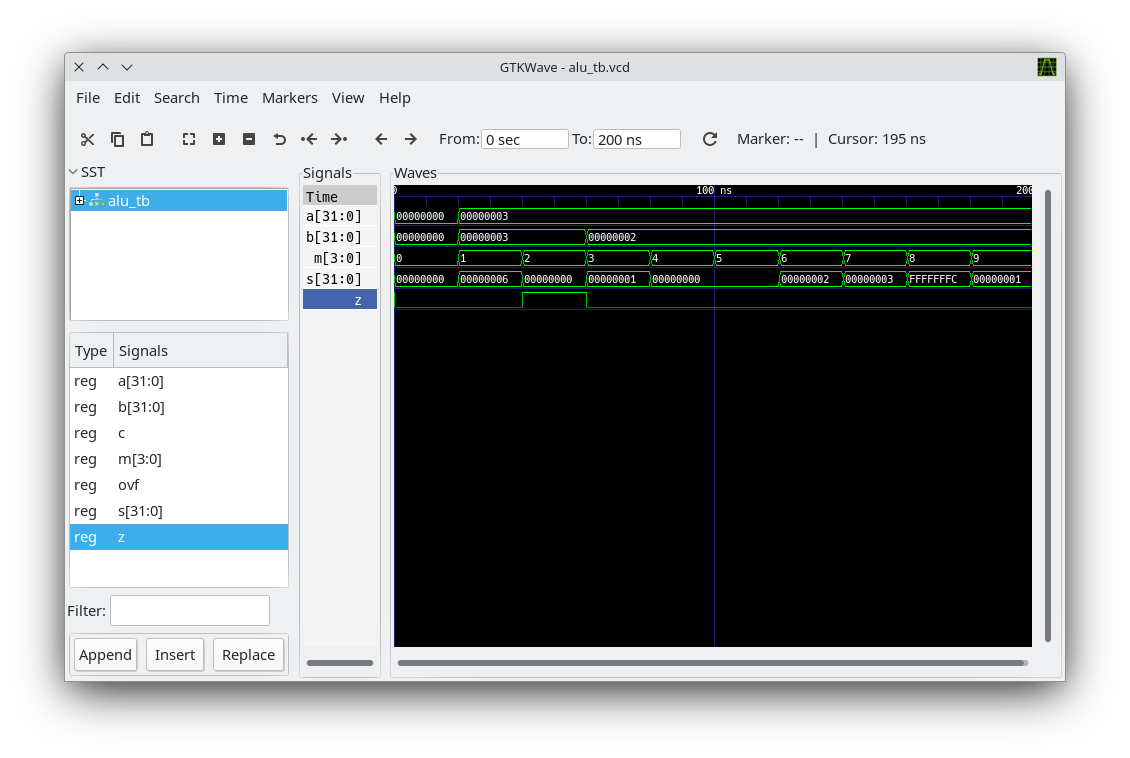
\includegraphics[width=0.7\textheight, height=\textwidth, angle=90]{signals}
\end{center}
\end{document}